\section{Toolchain}

MARK II is not only SoC, there is also several tools that will help you to
write software for MARK II. They are writen in Python and are placed in tools
directory. Tools are primary intended for using under linux with python 2.7.
Typical workflow is on image \ref{fig:toolchain_workflow}, and tools consist
from following parts.

\begin{itemize}
    \item \textbf{Assembler} - translate programs from symbolic language into machine code
    \item \textbf{Linker} - link multiple object files into loader module
    \item \textbf{Emulator} - emulate part of the SoC
    \item \textbf{Disassembler} - disassemble programs from machine code
    \item \textbf{ldm2mif} - script that convert loader module into mif and also can perform relocation
    \item \textbf{Loader} - perform relocation and load program into memory with serial bootloader
\end{itemize}

\begin{figure}[]
    \centering
    \includegraphics[width=.7\textwidth]{img/toolworkflow.png}
    \caption{MARK-II Toolchain - typical workflow}
    \label{fig:toolchain_workflow}
\end{figure}

\subsection{Assembler}

Simple two pass assembler for MARK-II is written in python 2.7 and is tested
under Linux. Assembler have basic support for macros and conditional translation.
In combination with linker, this simple assembler is able to do everything you
need, for development.

\subsubsection{Preprocessor}

Assembler have build-in preprocessor. This preprocessor have one pass
architecture, due this it isn't able to perform any forward declarations and any
recursions in macros. Preprocessor have build-in following commands:

\begin{itemize}
    \item \textbf{\#define symbol} -
    Define an symbol that is used ONLY with conditional assembly.

    \item \textbf{\#ifdef symbol} -
    If symbol is defined, assembler will parse following code, otherwise code
    will be skipped to the nearest \#endif. Note: "\#if" block can be nested.

    \item \textbf{\#ifndef symbol} -
    Same as \#ifdef but assembly code when symbol does not exist.

    \item \textbf{\#endif} -
    Identify end of condition assembly block.

    \item \textbf{\#include file} -
    Include file into current buffer.

    \item \textbf{\#macro name parms} -
    Define an new macro, everithing up to \#endmacro will be body of new macro.

    \item \textbf{\#endmacro} -
    Close macro body and write it into macro table.
\end{itemize}

\subsubsection{Macros}

Macro is small sequence of code that can be simple defined once and pasted into
code many times. Lets say there is an macro called "setLed". You can invoke it
with code like this:

\begin{lstlisting}[language={[x86masm]Assembler}, frame=single]
    $setLed
\end{lstlisting}

Prefix \$ is mandatory when invoking macro and tell the preprocesor "I wan't
paste macro setLed here!". Preprocesor then take body of setLed macro and paste
it into output buffer.

Macro can be defined using \#macro and \#endmacro preprocesor commands. For
example we will define macro setLed.

\begin{lstlisting}[language={[x86masm]Assembler}, frame=single]
    #macro setLed
        MVIL R1 0x0001
        ST R1 PORTA
    #endmacro
\end{lstlisting}

Macros can have arguments in ther definition. This feature is used in same way
as argument in C functions. For first you have to define macro with argument in
name. Let's say we want an macro "send" for sending by urat. This macro will
have one argument - byte to send. Code should look something like this:

\begin{lstlisting}[language={[x86masm]Assembler}, frame=single]
    #macro send byte
        ;some code for prepare sending
        ST byte UDR0
    #endmacro
\end{lstlisting}

Well, now we have macro defined, we will use it somewhere in the code like this:

\begin{lstlisting}[language={[x86masm]Assembler}, frame=single]
    $send 0xAA
\end{lstlisting}

Value "0xAA" will be automaticaly placed everywhere "byte" is written, when
macro is invoking.

Assembler have build in support for labels inside macros. This mean, you can
define label in macro and then call it. But this feature have exception that
normal labels doesn't.

You can call label only within macro definition itself. There is no way to call
label defined inside macro from normal code. This is because when you invoke
macro, labels get automatically renamed. There is unique name for each instance
of macro.

See example bellow to get this clear.

\begin{lstlisting}[language={[x86masm]Assembler}, frame=single]
    ;define new macro for delay

    #macro delay time
        .MVI R1 time
        loop:
        DEC R1 R1
        CMP EQ R1 R0 R2
        BZ R2 loop
    #endmacro

    ; some usefull code is here
    OR R0 R0 R0

    $delay 100      ; invoke macro "delay"

    ; assembler take definition of delay macro - replace loop "label" with "loop1"
    ; (1 because this is first instance of this macro) - and place macro body there

    ; there is another tons of usefull code
    OR R0 R0 R0

    $delay 1000     ; next instance of delay - now "loop2" is created
\end{lstlisting}

But macros also have some limitations. Mainly:

\begin{itemize}
    \item Macros can't be nested.
    \item Macro have to be complete defined before invoking.
    \begin{itemize}
        \item This also mean any recursion.
    \end{itemize}
\end{itemize}

\subsubsection{Numbers}

Numbers are parsed in C like form so:

\begin{itemize}
    \item \textbf{0x10} - hexadecimal number, 16 in decimal form
    \item \textbf{0b1010} - binary number, 9 in decimal form
    \item \textbf{74} - decimal number 74
\end{itemize}

\subsubsection{Labels}

When they are defined, they have to be followed with semicollon ':'. When used
(eg. with CALL instruction), semicollon is not used anymore. Example code:

\begin{lstlisting}[language={[x86masm]Assembler}, frame=single]
    halt:
        OR R0 R0 R0
        BZ R0 halt
\end{lstlisting}

\subsubsection{PseudoInstructions}

They have to start with dot '.'. They are used for controlling assembler. Following
PseudoInstructions are supported:

\begin{itemize}
    \item \textbf{.CONS name value} -
    Set constant <name> with contain <value>. Assembler simply replace all
    <name> in source code with <value>. This is not an macro and only numeric
    values can be processed!

    \item \textbf{.ORG value} -
    Set location counter to specified location during pass1.

    \item \textbf{.DAT word*} -
    Reserve space in memory at current location with size for all words.
    Memory is then filled with them. Every word have to be separed with
    space.

    \item \textbf{.DS size} -
    Only reserve space in memory at current location with size <size> in words.

    \item \textbf{.EXPORT name} -
    Export label for use in another object file. This pseudoinstruction create
    an special symbol. Special symbols are then printed into object file for
    linker.

    \item \textbf{.IMPORT name} -
    Import exported label from another object file. This pseudoinstruction
    create an special symbol. Special symbols are then printed into object file
    for linker.

    \item \textbf{.MVI register value} -
    Load register with 32b value. This is usefull when you want load constants
    into registers.
\end{itemize}

\subsection{Emulator}

Emulator is great way to test your codes and get in touch with MARK II without
use of FPGA.

Whole emulator is written in python only. This include SoC too. You can run
MARK II emulator in two modes, in CLI mode and GUI mode.

CLI mode is more simple, you just specify what MIF load into ROM0 and where to
connect UART0 and done. Emulator then start code in ROM0 like real hardware
does. You didn't see any result but you can communicate with CPU using UART and
for example socat with some serial terminal.

GUI mode is great for debugging purposes. GUI is written in tkinter and is
relative simply. But contains all what is needed for debugging. You can step
your program. You can view all memories, all registers, set breakpoint and run
to it. Also you can see disassembled content of memory.

Remember, not whole SoC is emulated. Emulated peripherals are only these what
is important. This mean:

\begin{itemize}
   \item cpu0
   \item rom0 - CPU start execution from here
   \item ram0 - on FPGA this is fastest ram
   \item ram1 - on FPGA this will become external SDRAM soon (at this time is implemented in same way as ram0)
   \item intController - is neccecery for CPU
   \item uart0 - we want some way to comunicate (work only at 9600 8N1, ignoring all settings)
\end{itemize}

\subsubsection{How one can work with CLI emulator?}

Simply, write your code in .asm file, translate it and link it into loadable
module (.ldm), the use utility ldm2mif and generate mif file for rom0.
Something like this.

\begin{lstlisting}[language=bash, frame=single]
    $ vim main.asm
    $ assembler --skip-linker main.asm
    $ ldm2mif main.ldm
    $ ls
    main.asm main.ldm main.mif
\end{lstlisting}

Now, you have to decide where to bind UART0, lets say, we want virtual serial
port to connect it like when real hardware is connected. Best way to do on
Linux is use socat and pty.

\begin{lstlisting}[language=bash, frame=single]
    $ socat -d -d pty,raw,echo=0 pty,raw,echo=0
    2017/06/02 11:41:50 socat[2252] N PTY is /dev/pts/1
    2017/06/02 11:41:50 socat[2252] N PTY is /dev/pts/2
    2017/06/02 11:41:50 socat[2252] N starting data transfer loop with FDs [5,5] and [7,7]
\end{lstlisting}

As you can see, we get two serial port /dev/pts/1 and /dev/pts/2. They are
connected together with "virtual null modem cable". So, we open can listen on
pts/2 and connect emulator to pts/1. For listening we can use cat.

\begin{lstlisting}[language=bash, frame=single]
    $ cat /dev/pts/2
\end{lstlisting}

And now is time to run your emulator.

\begin{lstlisting}[language=bash, frame=single]
    $ emulator -p /dev/pts/1 -r main.mif
    MARK-II GUI emulator v0.1.9_1
    UART0 mapped into "/dev/pts/1"
    ROM0 loaded with "main.mif"
    For exit from emulator please use CTRL+C.
\end{lstlisting}

That is all. If you want to exit, use CTRL+C.

\subsubsection{How one can work with GUI emulator?}

This is almost same as CLI. So, create your mif in same way.

\begin{lstlisting}[language=bash, frame=single]
    $ vim main.asm
    $ assembler --skip-linker main.asm
    $ ldm2mif main.ldm
    $ ls
    main.asm main.ldm main.mif
\end{lstlisting}

Open pair of serial ports. (note: you can use real port, just give emulator as
parameter something like /dev/ttyUSB0)

\begin{lstlisting}[language=bash, frame=single]
    $ socat -d -d pty,raw,echo=0 pty,raw,echo=0
    2017/06/02 11:41:50 socat[2252] N PTY is /dev/pts/1
    2017/06/02 11:41:50 socat[2252] N PTY is /dev/pts/2
    2017/06/02 11:41:50 socat[2252] N starting data transfer loop with FDs [5,5] and [7,7]
\end{lstlisting}

Listen on the port.

\begin{lstlisting}[language=bash, frame=single]
    $ cat /dev/pts/2
\end{lstlisting}

And run emulator.

\begin{lstlisting}[language=bash, frame=single]
    $ emulator -g -p /dev/pts/1 -r main.mif
    MARK-II GUI emulator v0.1.9_1
    UART0 mapped into "/dev/pts/1"
    ROM0 loaded with "main.mif"
\end{lstlisting}

New window appear, you can see GUI at image \ref{fig:gui_emulator}. Controlling
is simple. Use tick button to execute one instruction, use reset to reset SoC
and exit to exit from emulator. "Run to" can be used for breakpoint. And you
should see memories contents and also registers contents.

\begin{figure}[h]
    \centering
    \includegraphics[width=\textwidth]{img/emulator.png}
    \caption{MARK-II GUI Emulator}
    \label{fig:gui_emulator}
\end{figure}

\subsection{Usage}

\subsubsection{Assembler}

\begin{lstlisting}[language=bash, frame=single]
    Example usage: assembler main.asm

    Arguments:
        -h --help           Print this help.
        -o --output         Output object file name.
           --skip-linker    Generate relocatable loader module
                            instead object file. Can be used for
                            skipping linker if linking is not needed.
           --version        Print version number and exit.
\end{lstlisting}

Assembler take one file with ".asm" and translate it into object file ".o".
Object files are then readed by linker and linked together into loadable module
".ldm". You can skip linker step by specifying "--skip-linker" argument.

Please note, if you use preprocessor directive "\#include file.asm", you don't
need this file linked, because preprocessor take whole "file.asm" and paste it
into current file. Linker is needed when you used pseudo-instruction ".IMPORT
label".

\subsubsection{Linker}

\begin{lstlisting}[language=bash, frame=single]
    Example usage: linker example1.o example2.o

    Arguments:
        -h --help           Print this help.
        -o <file>           Output LDM file name. If not specified,
                            name of first object file will be used.
           --version        Print version number and exit.
\end{lstlisting}

Link multiple object files into one loadable module. Linker is necessary when
you split your code into multiple files and use ".EXPORT label" and ".IMPORT
label" pseudo-instructions.

In that case just compile each file separated and then call:

\begin{lstlisting}[language=bash, frame=single]
    # linker file1.o file2.o
\end{lstlisting}

\subsubsection{ldm2mif}

\begin{lstlisting}[language=bash, frame=single]
    Example usage: ldm2mif example.ldm

    Arguments:
        -h --help           Print this help.
        -o <file>           Output MIF name. If not specified name of
                            input file will be used.
        -r <address>        Relocate source. Add just immediate
                            addresses of these instructions that use
                            relative addressing using labels.
                            You have to specify <address> in hex
                            where the code will be stored. Default
                            value is 0x000000.
        -s <size>           Size of memory, default value is 8.
                            Memory range is from 0 to 2^<size>.
           --version        Print version number and exit.
\end{lstlisting}

This simple tool is used to convert loadable module into ".mif" files for
Quartus. You can specify size of memory and also base address of memory. All
relative symbols (like jump into labels) will be recalculated relative to the
base address.

\subsubsection{disassembler}

\begin{lstlisting}[language=bash, frame=single]
    Example usage: disassembler uart.ldm

    Arguments:
        -h --help           Print this help.
        -o --output         Output file name.
           --version        Print version number and exit.
\end{lstlisting}

Read compiled loadable module and translate it back to assembler source codes.

\subsubsection{loader}

\begin{lstlisting}[language=bash, frame=single]
    Example usage: loader -b 0x400 -p /dev/ttyUSB0 example.ldm

    Arguments:
        -h --help           Print this help.
        -b <address>        Base address, using hex C like syntax,
                            to store source.
                            Loader also perform relocation of the
                            given source to this address.
        -p <port>           Port where MARK-II is connected. For
                            example /dev/ttyUSB0.
           --baudrate       Set baudrate for port. Default value is
                            1200.
           --version        Print version number and exit.
\end{lstlisting}

Simple tool for loading programs into CPU using UART. Simply specify the base
address where you want store your code, specify port where MARK-II is connected
and wait. MARK-II must be connected before sending started.

\subsubsection{emulator}

\begin{lstlisting}[language=bash, frame=single]
    Example usage: emulator -g -p /dev/pts/2 -r rom.mif

    Arguments:
        -h --help           Print this help and exit.
        -p --port           Device where uart0 will be connected.
                            Can be /dev/pts/2 for example.
        -r --rom            Filename of file that will be loaded
                            into rom0.
        -g --gui            Run with simple GUI.
           --version        Print version number and exit.
\end{lstlisting}

Great way to test your program and get in touch with MARK-II. Enable execution
of programs in almost same way like real HW. Also emulate uart0 so you can
connect serial port monitor.


